\section{Desarrollo}

\subsection{solver_lin_solve}

Como primer enfoque para la implementación de {\it solver_lin_solve\/} se pensó en
leer de a columnas y maximizar la cantidad de posiciones que calculábamos a
la vez, tal como puede apreciarse en la \hbox{\it figura 1\/}.

La principal ventaja de leer de a columnas, es reusar la fila calculada con
anterioridad, evitándose así una relectura a memoria.

Luego, para maximizar la cantidad de posiciones, se usaban los 16 registros {\it
  xmm\/}.
Dando por resultado la lectura de segmentos de matriz de $3\times24$
posiciones simultáneas y el calculo de 22 posiciones nuevas por iteración del
ciclo. En cada iteración se leían 24 posiciones nuevas de la siguiente fila
(siempre manteniéndose en la misma columna de 24 elementos).
Una vez que ya no era posible de a 24, se terminaba de iterar la matriz
calculando de a 2 posiciones.

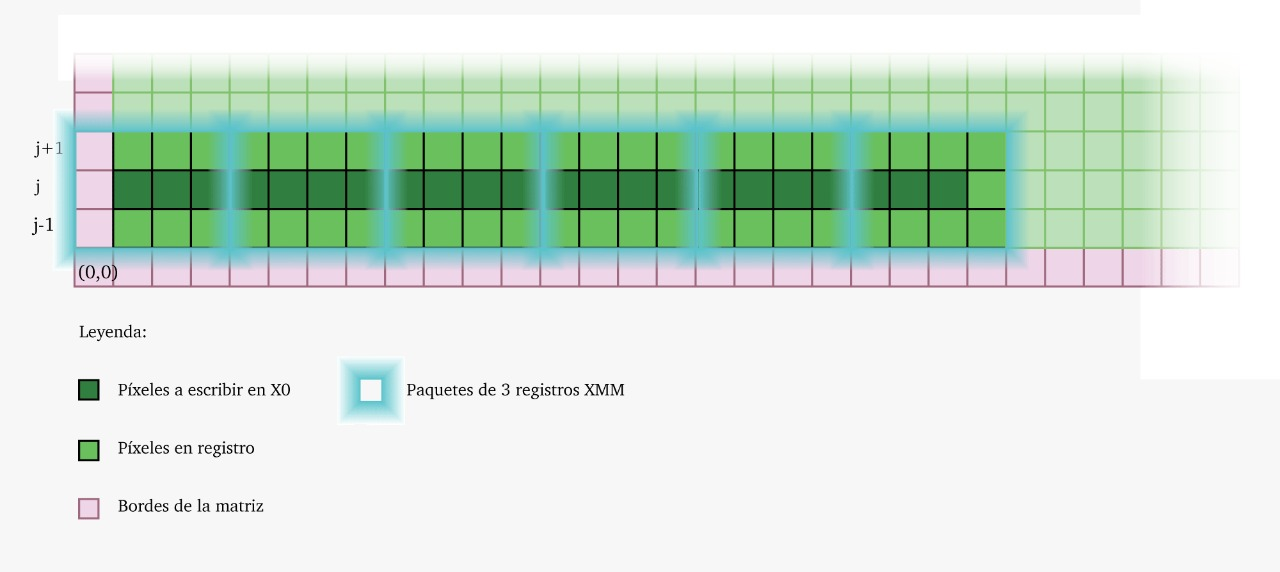
\includegraphics[width=\textwidth]{imagenes/24.jpeg}

Dicha implementación no fue completamente terminada, pero primeras
pruebas de la misma mostraron un rendimiento muy por debajo de lo esperado,
dando solo una leve mejora a la versión C provista por la cátedra (ver más en
resultados (sección piripitruli)).

Por este motivo fue descartada (código en {\it solver_lin_solve_largo.asm\/}
\footnote{El código no presenta errores de {\bf segmentation fault} y puede ser
  ejecutado. Sin embargo, al ser un código {\bf no} finalizado, produce errores
  en el cálculo de fluidos.}).

Entre las hipótesis acerca de la merma de rendimiento pensamos en la extensa
longitud del código de los ciclos y la forma de lectura por columnas de la
matriz que no aprovecha el modo de almacenamiento por filas \footnote{\#define
  IX(i,j) (i+(solver->N+2)*j)}.

\noindent\hfill\rule{0.7\textwidth}{0.4pt}\hfill
\hskip0.3em

Como opción final, se optó leer por medio de iteradores (puntero a la matriz)
que recorran la matriz por filas y calculen de a 2 posiciones a la vez,
$(i,j)$ e $(i+1,j)$.

Usándose la estrategia detallada a continuación para realizar el siguiente
calculo en paralelo, para cada posición de la matriz:

$$x(i,j) = \frac{x_0(i,j) +
  a*\bigl(x(i-1,j)+x(i+1,j)+x(i,j-1)+x(i,j+1)\bigr)}{c}$$

Primero notamos que si separamos en casos $a = 0$ y $a \neq 0$, nos permite que
en el caso $a = 0$, el cálculo se reduzca a:

$$x(i,j) = \frac{x_0(i,j)}{c}$$

Que podemos realizarlo de a 4 posiciones en paralelo por iteración de ciclo,
por medio de un iterador de $x_0$ y un iterador de $x$, en contraposición a
calcular de a 2 posiciones como realizamos en el caso general ($a \neq 0$), que
detallaremos más adelante. Otra ventaja es que el cálculo se reduce a una sola
instrucción (dividir por {\it c\/}).



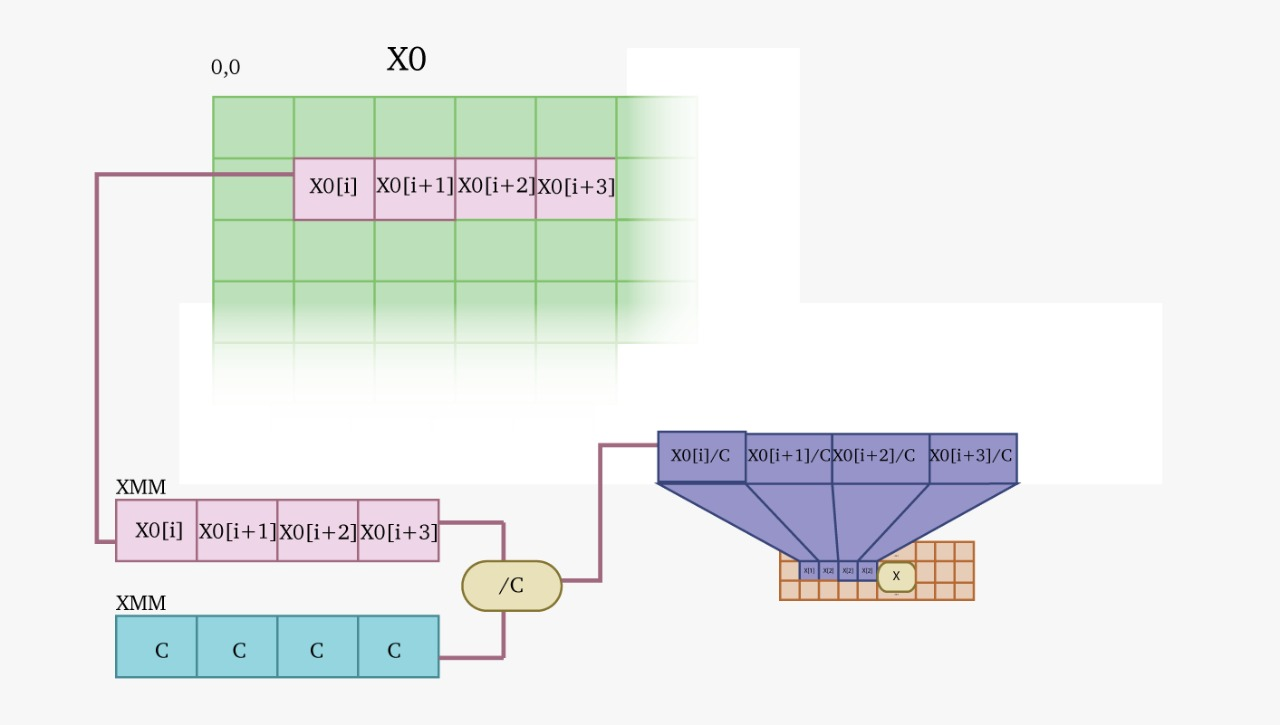
\includegraphics[width=\textwidth]{imagenes/lina0.jpeg}


x0 --> (carga en xmm) | x0[i][j] | x0[i+1][j] | x0[i+2][j] | x0[i+3][j] |
--> (div por c) | x0[i][j]/c | x0[i+1][j]/c | x0[i+2][j]/c | x0[i+3][j]/c |
--> (carga en memoria) x

En el caso $a \neq 0$, se utilizan 4 iteradores que apuntan respectivamente

% iter1_x: x(i,j-1)
% iter2_x: x(i-1,j)
% iter3_x: x(i,j+1)
% iter_x0: x0(i,j)



En cada iteración, se calculan las posiciones $x(i,j)$ y $x(i+1,j)$.
Se leen 2 posiciones a partir de {\it iter1_x\/}, 2 de {\it iter3_x\/}, 2 de
{\it iter_x0\/} y 4 de {\it iter2_x\/}, dando por resultado la carga en
registros {\it xmm\/} de las siguiente posiciones.

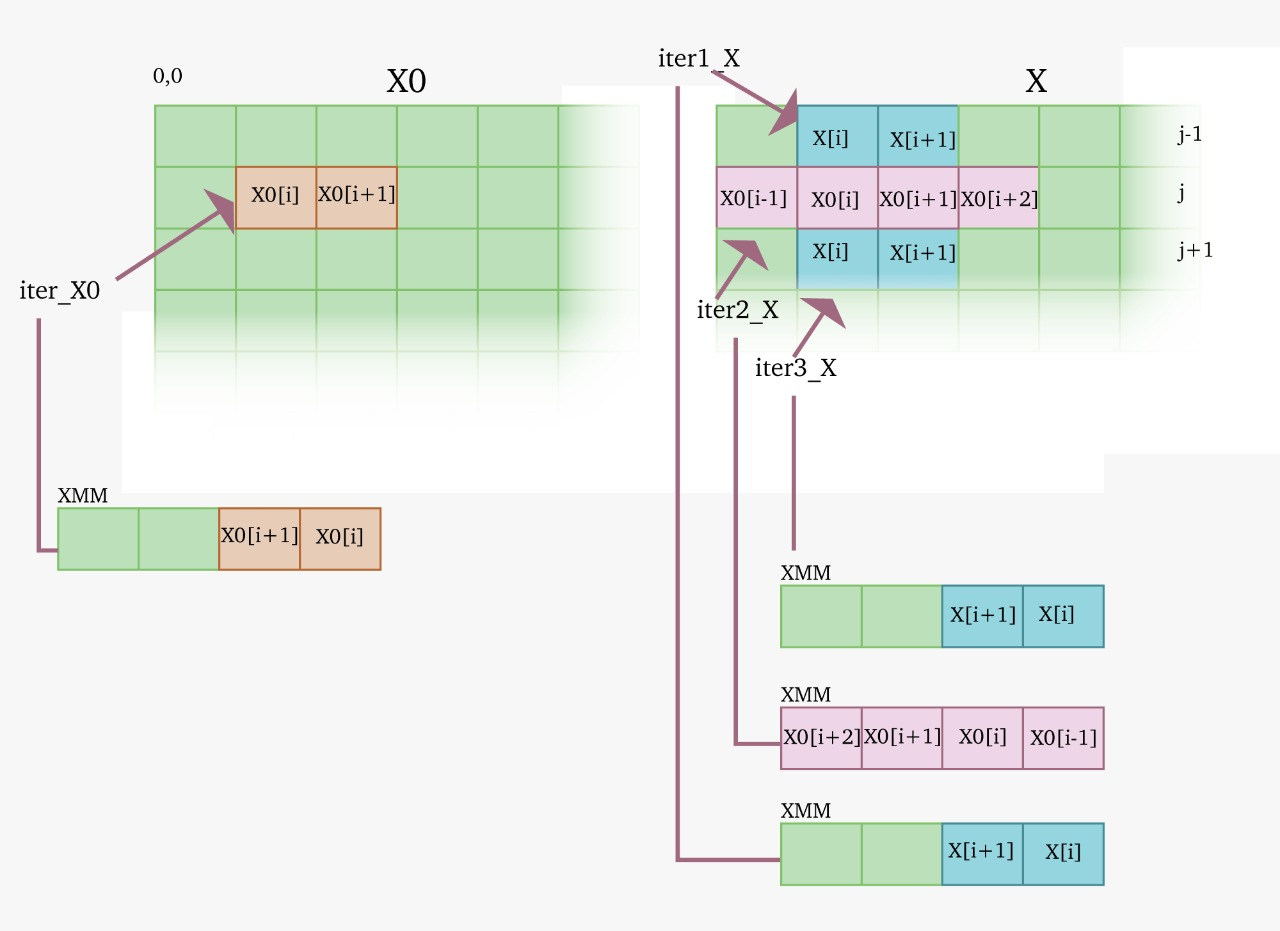
\includegraphics[width=\textwidth]{imagenes/liniter.jpeg}


Consecuentemente, se calculan en paralelo, es decir de a 2 posiciones
simultáneas, la suma

{
\setlength{\abovedisplayskip}{-5pt}
\setlength{\belowdisplayskip}{-5pt}
\begin{align*}
x(i,j) &:= \frac{x_0(i,j)}{a} + x(i+1,j) + x(i,j-1) + x(i,j+1)\\
x(i+1,j) &:= \frac{x_0(i,j)}{a} + x(i+1,j) + x(i,j-1) + x(i,j+1)
\end{align*}
}


para $x(i,j)$ y $x(i+1,j)$ como muestra la figura.

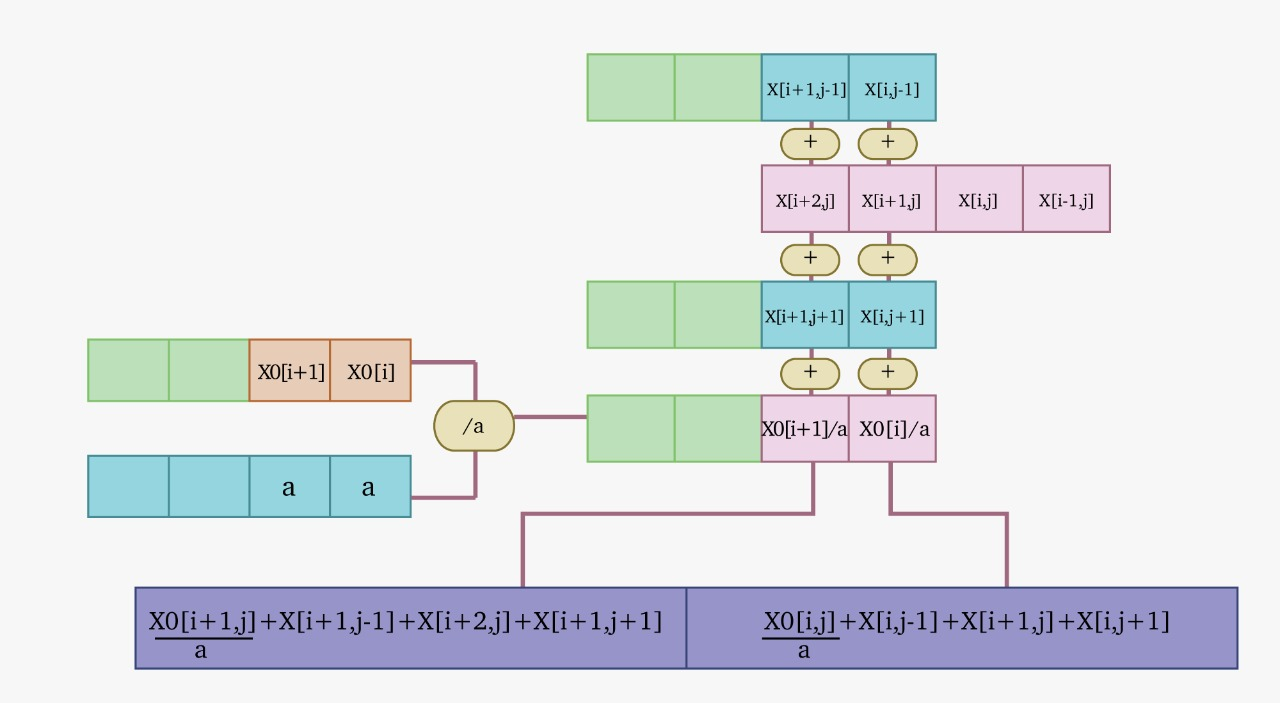
\includegraphics[width=\textwidth]{imagenes/lina11.jpeg}


Luego, se calcula secuencialmente
$$x(i,j) + x(i-1,j)$$
$$x(i,j) / c$$
$$x(i+1,j) + (i,j)$$
$$x(i+1,j) / c$$


FIGURA (diagrama que va mostrando los pasos del algoritmo)

Esto es necesario, debido a que cada posición necesita que la casilla a su
izquierda $x(i-1,j)$ haya sido procesada con anterioridad al sumarse a $x(i,j)$.

Vale la pena aclarar que la casilla $x(i,j-1)$ también debe haber sido procesada al
momento de su suma, pero debido a la manera en que se recorre la matriz, al
leerse la posición $x(i,j-1)$, ya fue calculada con anterioridad.

Por último, se incrementan en dos posiciones los iteradores y se sigue con una
nueva iteración del ciclo hasta completar la matriz.


Esta solución, en principio menos óptima ya que debía leerse 3 veces cada
posición de memoria (ver figura tanto), aprovecha mucho mejor el principio de
localidad en caché, tanto para el código (al ser mucho más compacto), como para
los datos (al recorrer la matriz por filas).

Quedó en el tintero aclarar el por qué las posiciones de memoria se leen 3
veces. Esto ocurre porque si en una iteración se leen las posiciones de $x$
$\bigl[(i,j)|(i+1,j)|(i+2,j)|(i+3,j)\bigr]$, en la siguiente se leen
$\bigl[(i+2,j)|(i+3,j)|(i+4,j)|(i+5,j)\bigr]$, releyéndose las posiciones
$\bigl[(i+2,j)|(i+3,j)\bigr]$. Luego las posiciones
$\bigl[(i+2,j-1)|(i+3,j-1)\bigr]$ también fueron calculadas anteriormente,
leyéndose por tercera vez.

FIGURA |x(i,j)|x(i+1,j)  |x(i+2,j)  |x(i+3,j)  |x(i+4,j)|x(i+5,j)|
                         |x(i+2,j-1)|x(i+3,j-1)|
(poner i+2 e i+3 de otro color que resalte)

Esta desventaja fue superada guardando $x(i+2,j)$ y $x(i+3,j)$ de la iteración
anterior en la parte baja del registro y cargando $x(i+4,j)$ e $x(i+5,j)$ en la parte
alta del registro con {\it movhps\/}\footnote{movhps: carga las posiciones 2 y 3
del registro $xmm = [3|2|1|0]$} sin ninguna modificación extra al algoritmo utilizado.

% Se descartó también la posibilidad de maximizar la cantidad de posiciones
% cargadas al mismo tiempo en los registros,


\subsection{solver_set_bnd}

Para la función {\it solver_set_bnd\/} se desglosó el ciclo en casos $b = 1$,
$b = 2$ y $b \neq 1 \land b \neq 2$.

Al hacerlo, se evita realizar comparaciones dentro del ciclo. Quedando por
resultado un ciclo que por cada iteración calcula lo siguiente:

\begin{center}
  \begin{tabular}{| >{\centering\arraybackslash}m{2in} | >{\centering\arraybackslash}m{2in} | >{\centering\arraybackslash}m{2in} |}
    \hline
    $b = 1$              & $b = 2$              & $b \neq 1 \land b \neq 2$ \\\hline
{
\setlength{\abovedisplayskip}{0pt}
\setlength{\belowdisplayskip}{0pt}
\begin{align*}
  x(0,i) &:= -x(1,i)\\ x(n+1,i) &:= -x(n,i)\\  x(i,0) &:= x(i,1)\\ x(i,n+1) &:= x(i,n)
\end{align*}
} & {
\setlength{\abovedisplayskip}{0pt}
\setlength{\belowdisplayskip}{0pt}
\begin{align*}
  x(0,i) &:= x(1,i)\\ x(n+1,i) &:= x(n,i)\\ x(i,0) &:= -x(i,1)\\ x(i,n+1) &:= -x(i,n)
\end{align*}
} & {
\setlength{\abovedisplayskip}{0pt}
\setlength{\belowdisplayskip}{0pt}
\begin{align*}
  x(0,i) &:= x(1,i)\\ x(n+1,i) &:= x(n,i)\\  x(i,0) &:= x(i,1)\\ x(i,n+1) &:= x(i,n)
\end{align*}} \\\hline
  \end{tabular}
\end{center}

Se usan 4 iteradores y 1 ciclo que itera n veces, calculándose por cada
iteración una nueva posición.
Estos iteradores son {\it upper\/}, {\it bottom\/}, {\it left\/} y {\it right_n\/}.
Y recorren respectivamente,

FIGURA (cuadrito con bordes y nombres del iterador en cada uno)

Por último se realizan los últimos calculos de la misma forma que el código
original

{
\setlength{\abovedisplayskip}{-5pt}
\setlength{\belowdisplayskip}{-20pt}
\begin{align*}
  x(0  ,0  ) &:= 0.5\cdot\bigl(x(1,0  )+x(0  ,1)\bigr)\\
  x(0  ,n+1) &:= 0.5\cdot\bigl(x(1,n+1)+x(0  ,n)\bigr)\\
  x(n+1,0  ) &:= 0.5\cdot\bigl(x(n,0  )+x(n+1,1)\bigr)\\
  x(n+1,n+1) &:= 0.5\cdot\bigl(x(n,n+1)+x(n+1,n)\bigr)\\
\end{align*}
}

Notar que se usa un iterador {\it upper_n\/} ubicado en la fila $n$ en vez
de la $n+1$, esto es debido al formato en que pueden indexarse las direcciones
en {\it intel\/} donde solo se pueden sumar registros y no restarse. En el caso
de haberse optado por un iterador de la fila $n+1$, la siguientes líneas
\footnote{Línea 120 y 121, {\it solver_set_bnd.asm\/}}

\lstset{numbers=none}
\begin{lstlisting}
  mov aux_edx, [upper_n]            ; aux := x[i][N]
  mov [upper_n + lon_fila], aux_edx ; x[i][N+1] := x[i][N]
\end{lstlisting}
deberían ser idealmente
\begin{lstlisting}
  mov aux_edx, [upper - lon_fila]   ; aux := x[i][N]
  mov [upper], aux_edx              ; x[i][N+1] := x[i][N]
\end{lstlisting}

Como la operación no está permitida, la resta debería realizarse anteriormente
en un registro auxiliar. Para evitar esto y aprovechar el modo de
direccionamiento de {\it intel\/}, usamos un iterador a la posición $n$.


\subsection{solver_project}

En esta función se utilizó la misma forma de recorrer la matriz por filas
adoptada en {\it solver_lin_solve\/} (ver blabla), los motivos son los mismos,
aprovechar el principio de localidad en caché.

El calculo a realizar es

{
\setlength{\abovedisplayskip}{-5pt}
\setlength{\belowdisplayskip}{-10pt}
\begin{align*}
  div(i,j) &:= \frac{-0.5 \cdot \bigl(u(i+1,j)-u(i-1,j)+v(i,j+1)-v(i,j-1)\bigr)}{n}\\
  p(i,j)   &:= 0
\end{align*}
}

En primer lugar, para el primer ciclo se utilizan los iteradores {\it div\/},
{\it u\/}, {\it v1\/} y {\it v2\/}.
% FIGURA iteradores
% div: div(i,j)
% u: u(i-1,j)
% v1: v(i,j-1)
% v2: v(i,j+1)
Y se calcula de a 2 posiciones por iteración. Leyendo 4 posiciones de {\it u\/},
2 de {\it v1\/} y 2 de {\it v2\/}. Realizando el cálculo como indica la figura,

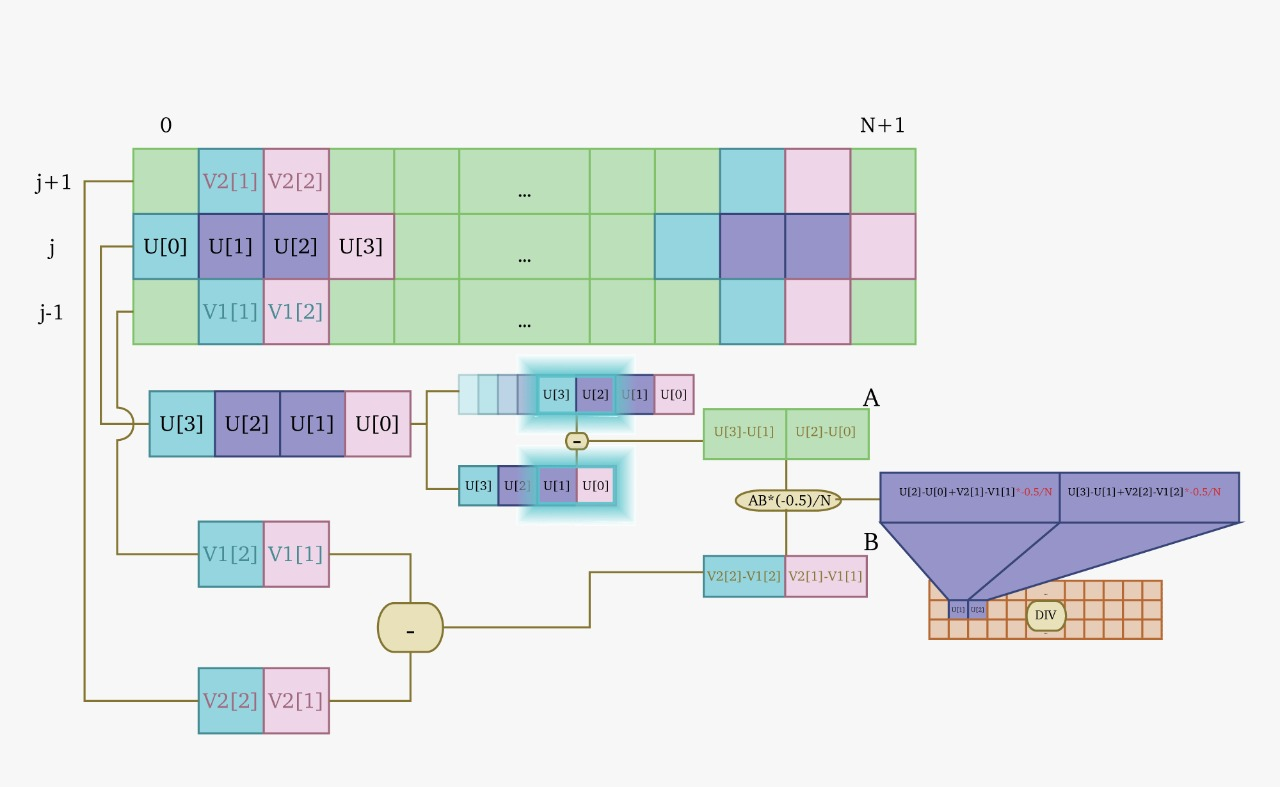
\includegraphics[width=\textwidth]{imagenes/div.jpeg}

Por último, se incrementan los iteradores en 2 posiciones y se da paso a la
siguiente iteración.

Para el segundo ciclo, donde debe calcularse

{
\setlength{\abovedisplayskip}{-5pt}
\setlength{\belowdisplayskip}{-10pt}
\begin{align*}
  u(i,j) &:= u(i,j) - 0.5n\cdot\bigl(p(i+1,j)-p(i-1,j)\bigr)\\
  v(i,j) &:= v(i,j) - 0.5n\cdot\bigl(p(i,j+1)-p(i,j-1)\bigr)
\end{align*}
}

se optó por separar el ciclo en dos diferentes, en el primero se calcula
{\it u\/} y en el segundo se calcula {\it v\/}.

Esto conlleva la ventaja de poder calcular de a 4 posiciones en paralelo para
{\it v\/} y sortear la limitación de calcular de a 2 posiciones debido al
calculo de {\it u\/} como se explicará a continuación.

La estrategia utilizada para el ciclo de {\it u\/} es usar 2 iteradores, {\it
  iter_p\/} e {\it iter_u\/}.

% iter_p: p[i-1][j]
% iter_u: u[i][j]

\begin{center}
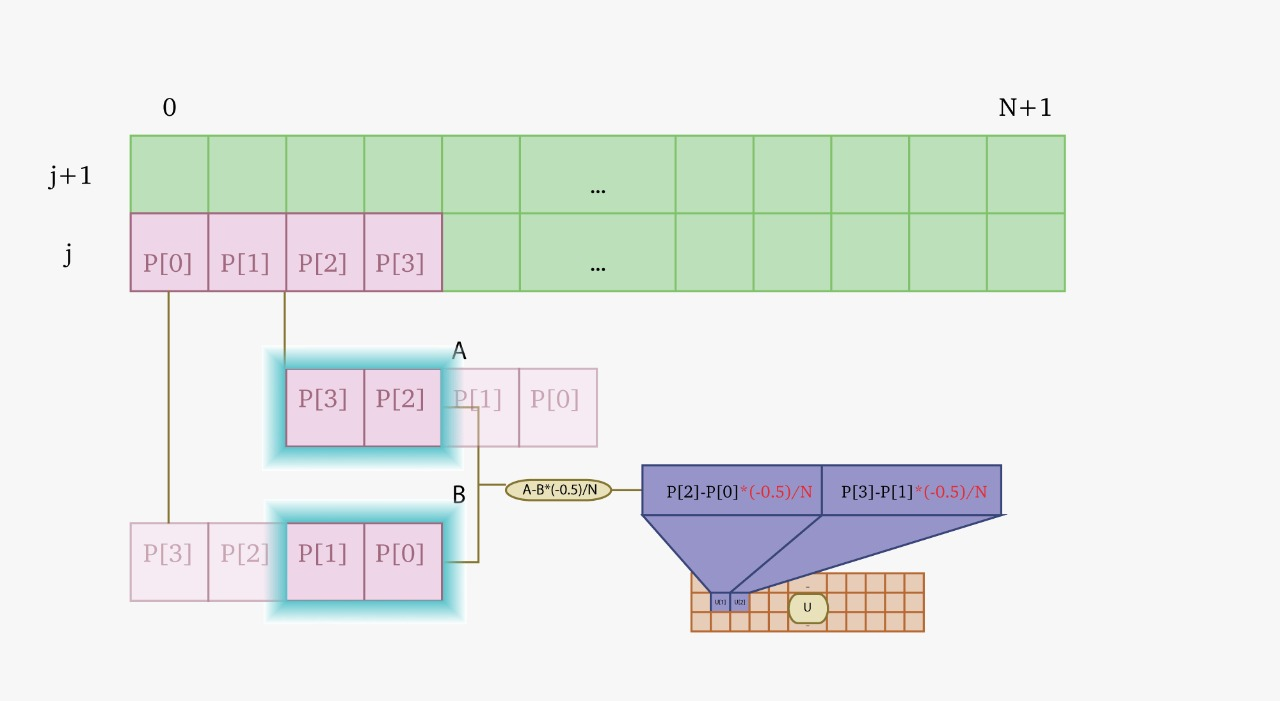
\includegraphics[width=0.7\textwidth]{imagenes/u.jpeg}
\end{center}

En cada iteración se leen 4 posiciones de {\it p\/} y se procesan 2 posiciones
de {\it u\/}.

Diagrama (muestra como calcula paralelamente u)

La estrategia utilizada para el ciclo de {\it v\/} es usar 3 iteradores, {\it
  iter1_p\/}, {\it iter2_p\/} e {\it iter_v}.

% iter1_p: p[i][j-1]
% iter2_p: p[i][j+1]
% iter_v: v[i][j]

Figura (muestra donde se ubican los iteradores)

En cada iteración se leen 4 posiciones de {\it p\/}, 4 de {\it p\/} y se
procesan 4 posiciones de {\it u\/}.

Diagrama (muestra como calcula paralelamente v)
